\chapter{Weitere Prinzipien}

\section{Analyse GRASP: Geringe Kopplung}

\textbf{Klasse: \code{Filereader}} (\code{header/filereader.hpp})

Die Klasse \code{Filereader} hat eine minimale Kopplung zu anderen Klassen. Sie bietet eine einzige öffentliche Methode \code{readFile(filename) -> tuple<bool, string>}, die eine Datei liest und den Inhalt zurückgibt. Sie hat keine Abhängigkeiten zu PIC-spezifischen Klassen.

\textbf{Aufrufer:} Nur die Klasse \code{Program} nutzt \code{Filereader} in der Methode \code{loadProgram()}. Ebenso nutzt \code{TUI_Controller} sie indirekt über \code{Program}. Da \code{Filereader} nur Standard-C++-Bibliotheken verwendet und keine PIC-spezifischen Typen kennt, kann sie problemlos wiederverwendet oder ausgetauscht werden. Die Kopplung ist gering, weil:

\begin{itemize}
    \item Nur 1 Nutzer (\code{Program}) ist direkt abhängig
    \item Keine Kenntnis über die Domäne (PIC-Simulation)
    \item Rückgabewert ist ein generischer Typ (\code{tuple<bool, string>})
    \item Keine Abhängigkeiten zu anderen Projektklassen
\end{itemize}

\begin{center}
    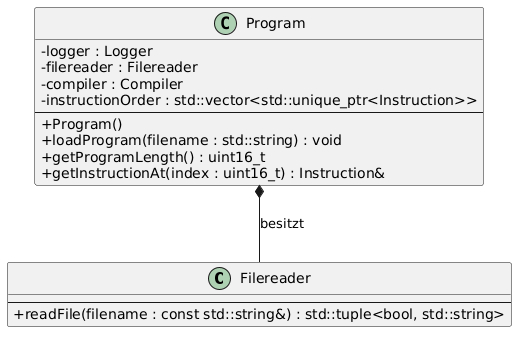
\includegraphics[width=0.9\textwidth]{UML/10.png}
\end{center}


\section{Analyse GRASP: Pure Fabrication}

\textbf{Klasse: \code{Logger}} (\code{header/logger.hpp})

Die Klasse \code{Logger} ist ein \textbf{Pure Fabrication} -- sie repräsentiert kein Konzept aus der PIC-Hardware-Domäne, sondern wurde ausschließlich aus softwaretechnischen Gründen erstellt, um eine einheitliche Logging-Infrastruktur bereitzustellen.

\textbf{Begründung des Einsatzes:} Ohne den Logger müsste jede Klasse ihre eigene Ausgabe-Logik implementieren (z.B. \code{std::cout}-Aufrufe), was zu Codeduplizierung führen würde. Der Logger bündelt die Verantwortlichkeit der Protokollierung an einer Stelle und bietet:

\begin{itemize}
    \item Konfigurierbare Log-Level (\code{INFO}, \code{ERROR}, etc.)
    \item Benannte Logger-Instanzen (z.B. \code{"Compiler"}, \code{"PIC"})
    \item Möglichkeit, einzelne Logger zu deaktivieren (in \code{main.cpp})
\end{itemize}

Die Klasse gehört nicht zur Domäne, ist aber essenziell für die Wartbarkeit der Software.

\begin{center}
    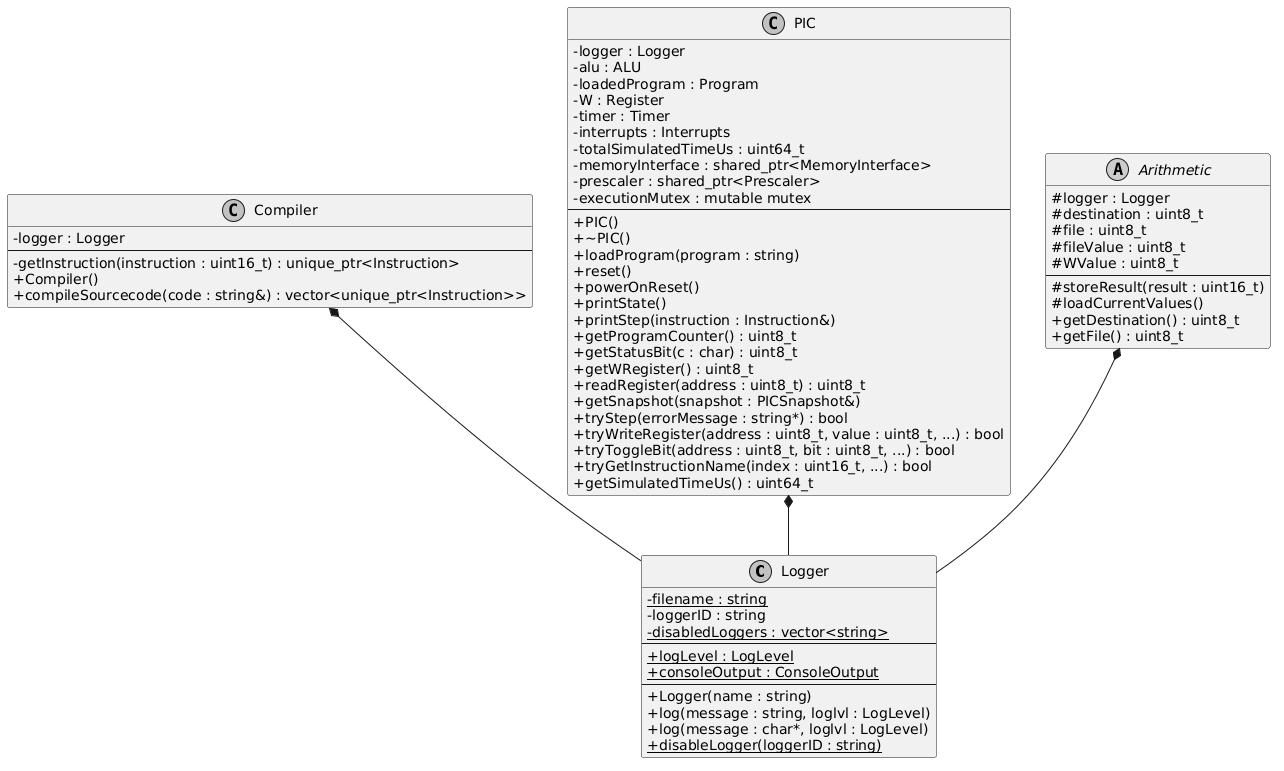
\includegraphics[width=0.9\textwidth]{UML/11.png}
\end{center}

\section{DRY}

\textbf{Beispiel: (Commit: ed2bead79cd82429ca9a1f6071dcb06d4e7ba7f0)} throwErrors Funktion in der Ram Klasse.

\textbf{Vorher (duplizierter Code):} Ohne die Funktion wurde in jeder anderen Funktion der identische Code ausgeführt, um Fehler zu erkennen.


\begin{lstlisting}[style=codeblock,language=picassocpp]
uint8_t Ram::readRegister(uint8_t address)
{
    if (isOutOfScope(address))
        throw std::runtime_error("Address out of range");

    if (!memory[readBankSelectBit()][address])
    {
        throw std::runtime_error("Nullpointer access at address 0x" +
                                 std::to_string(address));
    }

    return memory[readBankSelectBit()][address]->readByte();
}

uint8_t Ram::readRegister(uint8_t address, bool bank)
{
    if (isOutOfScope(address))
        throw std::runtime_error("Address out of range");

    if (!memory[bank][address])
    {
        throw std::runtime_error("Nullpointer access at address 0x" +
                                 std::to_string(address));
    }

    return memory[bank][address]->readByte();
}
\end{lstlisting}

\textbf{Nachher (DRY durch Funktionsauslagerung):}

\begin{lstlisting}[style=codeblock,language=picassocpp]
uint8_t Ram::readRegister(uint8_t address)
{
    throwErrors(address);
    return memory[readBankSelectBit()][address]->readByte();
}

uint8_t Ram::readRegister(uint8_t address, bool bank)
{
    throwErrors(address, bank);
    return memory[bank][address]->readByte();
}
\end{lstlisting}

\textbf{Auswirkung:} Die Fehlererkennung wird an einer lokalen Stelle durchgeführt und kann besser angepasst werden, ohne teile zu vergessen.

